\documentclass[12pt]{article}\usepackage{graphicx}
\graphicspath{{./figs/}}{}

\usepackage{amsmath,amssymb,amsfonts,amsthm}
\newcommand{\myvec}[1]{\ensuremath{\begin{pmatrix}#1\end{pmatrix}}}
%\providecommand{\norm}[1]{\lVert#1\rVert}3
\usepackage{listings}
\usepackage{watermark}
\usepackage{titlesec}
\usepackage{caption}
\let\vec\mathbf
\lstset{
frame=single, 
breaklines=true,
columns=fullflexible
}
\usepackage{atbegshi}% http://ctan.org/pkg/atbegshi
\AtBeginDocument{\AtBeginShipoutNext{\AtBeginShipoutDiscard}}
\let\vec\mathbf
\providecommand{\norm}[1]{\left\lVert#1\right\rVert}
\providecommand{\qfunc}[1]{\ensuremath{Q\left(#1\right)}}
\providecommand{\sbrak}[1]{\ensuremath{{}\left[#1\right]}}
\providecommand{\lsbrak}[1]{\ensuremath{{}\left[#1\right.}}
\providecommand{\rsbrak}[1]{\ensuremath{{}\left.#1\right]}}
\providecommand{\brak}[1]{\ensuremath{\left(#1\right)}}
\providecommand{\lbrak}[1]{\ensuremath{\left(#1\right.}}
\providecommand{\rbrak}[1]{\ensuremath{\left.#1\right)}}
\providecommand{\cbrak}[1]{\ensuremath{\left\{#1\right\}}}
\providecommand{\lcbrak}[1]{\ensuremath{\left\{#1\right.}}
\providecommand{\rcbrak}[1]{\ensuremath{\left.#1\right\}}}
\newcommand{\solution}{\noindent \textbf{Solution: }}
\newcommand{\mydet}[1]{\ensuremath{\begin{vmatrix}#1\end{vmatrix}}}
\title{\mytitle}
\begin{document}
\begin{center}
\title{\textbf{VECTOR ALGEBRA}}
\maketitle
\end{center}
\begin{enumerate}
\item\textbf{Problem statement :} Find the area of a triangle with vertices
$
\vec{A} = \myvec{1\\1 \\2},
\vec{B} = \myvec{2\\3 \\5}, \text{ and }
\vec{C} = \myvec{1\\ 5\\5}
$
\\
\solution
From the given information, 
\begin{align}
\vec{B-A}=\myvec{2\\3\\5}-\myvec{1\\1\\2} = \myvec{1\\2\\3}\\
\vec{C-A}=\myvec{1\\5\\5}-\myvec{1\\1\\2}=\myvec{0\\4\\3}
\end{align}
The area of a triangle using the vector product is then obtained as
\begin{align}
        \frac{1}{2}\norm{\myvec{\vec{B-A}}\times\myvec{\vec{C-A}}} \\=\frac{1}{2}\norm{\myvec{1\\2\\3}\times \myvec{0\\4\\3}}
    \end{align}
Cross product of two vectors are  
 \begin{align}
      \vec{A}\times\vec{B} =\myvec{0&-A_3&A_2\\A_3&0&-A_1\\-A_2&A_1&0}\myvec{B_1\\B_2\\B3}
      \label{product}
\end{align}
By using \eqref{product}
\begin{align}
          \frac{1}{2}\norm{\myvec{\vec{B-A}}\times\myvec{\vec{C-A}}}=\frac{1}{2}\norm{\myvec{0&-3&2\\3&0&-1\\-2&1&0}\myvec{0\\4\\3}}\\
          =\frac{1}{2}\norm{\myvec{-6\\-3\\4}}\\
          =\frac{1}{2}\sqrt{(-6)^2+(-3)^2+(4)^2}\\
          =\frac{\sqrt{61}}{2}
\end{align}
\begin{figure}[!h]
 \begin{center}
  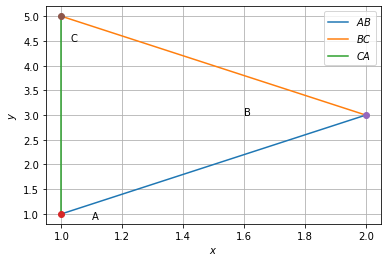
\includegraphics[width=\columnwidth]{figs/fig.png}
 \end{center}
\caption{}
\label{fig:Fig1}
\end{figure}
\end{enumerate}
\end{document}